%%% About this LaTeX template: %%%%%%%%%%%%%%%%%%%%%%%%%%%%%%%%%%%%%%%%%%%%%%%
%
% This template should work with any (reasonably recent) full
% installation of TeXLive or MikTeX. The "ecis2015" package loads a
% number of other packages, so if some package is missing, please
% install it using the package manager of your TeX distribution. In
% particular, if the "tikz" package is missing, you may have to install
% "pgf" or simply remove our example graphics (see figure example
% below).
%
% The file "ecis2015.sty" should be placed somewhere in your TeX Path
% (or simply in the same folder as your document).
%
% Please use PDFLaTeX to compile your document.
%
% You need not escape special characters or Umlauts like é ä ö ü ß (in 
% fact, you shouldn't), as this source is inputenc'd in UTF-8.
%
% Note for BibTeX users: We use BibLaTeX for formatting, so we use Biber
% as a sorting backend (default). 
% If you still need to use the old BibTeX program, please change the 
% BibLaTeX backend in the package file ("ecis2015.sty").
%
%%% Enter Document Info here: %%%%%%%%%%%%%%%%%%%%%%%%%%%%%%%%%%%%%%%%%%%%%%%%
\documentclass[a4paper,11pt,article,oneside]{memoir}
\usepackage{ecis2015}
\usepackage{url}
\usepackage{javascript_highlighting}
\usepackage{graphicx}
\usepackage{subfig}
\usepackage{multirow}
\usepackage{array}



\maintitle{Web 2.0 Projekt - Gruppenbildung} % ← Don't use UPPERCASE here, we do that automatically.
\shorttitle{Web 2.0 Projekt - Gruppenbildung} % ← This goes into the header.
\category{\url{https://groupfindr.herokuapp.com}} % ← Choose one by deleting the others.

\authors{% Separate authors by a "\par" or blank line.
\begin{tabular*}{1\linewidth}{@{\extracolsep{\fill}}c c c}
	Benedikt Bleyer & Fabio Isler & Genc Mazlami \\
 (14-706-162) & (09-115-965) & (09-923-061) \\
 \\
	Joel Scheuner & Moritz Schneider & Sebastian Stephan \\
 (10-741-494) & (11-490-455) & (08-731-465) \\
\end{tabular*}
}

\shortauthors{Bleyer, Isler, Mazlami, Scheuner, Schneider, Stephan} % ← This goes into the header. 

%%% BibTeX: %%%%%%%%%%%%%%%%%%%%%%%%%%%%%%%%%%%%%%%%%%%%%%%%%%%%%%%%%%%%%%%%%%

\addbibresource{bibliographie/literatur.bib} % ← Your .bib file, if you're using BibTeX
%\bibliography{bibliographie/literatur}

\newcommand{\code}[1]{\texttt{\small #1}}

\begin{document}

\renewcommand\thelstlisting{\arabic{lstlisting}}
\setcounter{lstlisting}{0}

%\begin{abstract}\noindent
Even if the development of the benefits management (BM) approach, which can be used to gain long-term benefits out of investments in information systems and information technology (IS/IT), was developed in 1996 the today's adoption rate in practice is low. By using components of a business intelligence (BI) platform as artefacts of a benefit management process the acceptance for the use of benefit management can be increased. To do so, it is important to follow specific design guidelines for a BI platform which are at least correlated with design principles and acceptance variables of benefits management itself.
\end{abstract}

%\begin{keywords}
  benefits management, business intelligence, acceptance research, design guidelines
\end{keywords}

\chapter{Hinführung und Problemstellung}
\label{kap1_hinfuehrung_problemstellung}


Test Test In vielen Lebenssituationen werden durch verschiedenen Individuen Gruppen gebildet. Hierbei existieren in der Literatur zahlreiche Definitionen für eine Gruppe. Nach Bierhoff und Frey ist eine Gruppe “eine Mehrzahl von Personen, die miteinander direkt interagieren und sich gegenseitig beeinflussen.”  \citep[Vgl.][S.~638]{bierhoff_handbuch_2006}
\newline\newline
Dabei können verschiedene Arten von Gruppen unterschieden werden.\citep[Vgl.][S.~11ff.]{thomas_grundris_1991} Es kann zum Beispiel zwischen einer Primärgruppe, wie die der Familie und Sekundärgruppen in Form von Arbeitsgruppen in einem Unternehmen differenziert werden. Mit Hilfe der Gruppengröße werden dabei zwischen Klein- und Großgruppen unterschieden. Eine Kleingruppe umfasst dabei maximal 30 Mitglieder, die der Großgruppe fasst maximal 100 Personen, da ansonsten keine direkte Interaktion gewährleistet ist. 
Häufig ist ebenfalls die Unterscheidung zwischen formellen und informellen Gruppen zu finden. \citep[Vgl.][S.~48]{spies_organisationspsychologie_2010}
Formelle Gruppen bekommen dabei die Ziele und die Regeln für die Zusammenarbeit von aussen vorgeben, bspw. der Universität oder dem Unternehmen vorgegeben. Ebenso sind den jeweiligen Gruppenmitgliedern einer formellen Gruppen spezifische Pflichten und Verantwortungen übertragen worden. Bei informellen Gruppen ist dies nicht der Fall und der Gruppe werden auch keine Ziele bzw. Aufgaben von aussen übertragen, vielmehr erfolgt die Bildung der informellen Gruppe bspw. aufgrund gleicher Bedürfnisse (bspw. die Begeisterung für die gleiche Fussballmannschaft). 
\newline\newline
Nach \citet{dick_teamwork_2013} ist ein Team "`eine Gruppe von Menschen, die gemeinsam an der Erreichung geteilter Ziele arbeiten, dabei verschiedene Rollen übernehmen und die miteinander kommunizieren, um so ihre Anstrengungen erfolgreich koordinieren zu können."' \citep[S.~1]{dick_teamwork_2013} Somit könnte ein Team als Teilmenge einer Gruppe angesehen werden, der Übergang ist jedoch fliessend. Daher wird auch vom "`Gruppe-Team-Kontinuum"' gesprochen.\citep[Vgl.][S.~14]{brettel_erfolgreiche_2009} In der vorliegenden Arbeit werden die Begriffe Gruppe und Team jedoch synonym gebraucht.
\newline\newline
Jede Gruppe durchläuft dabei die folgenden Phasen nach dem Modell von Tuckmann.\citep[Vgl.][S.~26-28]{dick_teamwork_2013} In der "`Forming"' Phase erfolgt ein erstes Abtasten und Kennenlernen der einzelnen Gruppenmitgliedern untereinandern. Die zweiten Phase ("`Storming"') ist durch Machtkämpfe sowie Streitigkeiten über die Regeln und Ziele innerhalb der Gruppe gekennzeichnet. Anschliessend erfolgt in der "`Norming"' Phase die Festlegung gemeinsame Ziele und Regeln für die Zusammenarbeit. Im ursprünglichen Modell war die "`Performing"' Phase die letzte Phase im Modell, in der die gemeinsame Arbeit zur Erreichung der festgelegten Ziele im Vordergrund steht. Später wurde das Modell jedoch durch die "`Adjourning"' Phase ergänzt, in der formelle Abschluss der Gruppentätigkeit und die anschliessende Auflösung im Vordergrund steht.
\newline\newline
Im Rahmen dieser Arbeit soll die Bildungsprozess der Gruppe durch eine Web-Anwendung erleichtert werden. Somit ist die Anwendung in der "`Forming"' Phase einzuordnen. Für die Gruppenart existieren theoretisch keine Beschränkungen, allerdings ist das graphische User-Interface (GUI) nur für Kleingruppen geeignet. Durch die Autoren wird die Anzahl von vier Gruppenmitglieder als optimal angesehen, ab acht Teilnehmer ist bereits die kritische Gruppengrösse erreicht. Die Idee für diese Art der Anwendung entstand durch die Problemstellung der Gruppenfindung für ein praktisches Projekt im Rahmen der Web 2.0 Vorlesung an der Universität Zürich im Frühlingssemester 2015.


\chapter{Konzept}
\label{konzept}

Das Ziel der Webanwendung ist die schnelle und einfache Bildung von Gruppen in Echtzeit. Das gewählte Konzept sieht als oberste Element den Raum vor. Der Raum kann bspw. im Kontext der Universität als das Äquivalent zu einer Vorlesung betrachtet werden. Die Anwendung erlaubt es jedem Benutzer beliebig viele Räume zu erstellen oder beliebig vielen bereits vorhandenen Räumen beizutreten. Sobald sich kein Benutzer mehr in einem Raum aufhält, wird der Raum gelöscht. Eine persistente Speicherung der Räume und/oder Gruppen mit deren Mitglieder ist nicht vorgesehen. 
\newline\newline
In jedem Raum können bis zu sieben Gruppen gebildet werden. Aktuell ist es jedem Benutzer gestattet eine neue Gruppe zu erstellen. Sobald sieben Gruppen erstellt wurden, erscheint jeweils eine Fehlermeldung, dass die maximale Anzahl der Gruppen bereits erreicht worden ist. Eine Beschränkung der Mitglieder pro Gruppe ist nicht vorhanden, allerdings wird die optimale Gruppengröße von vier bis sechs Mitgliedern durch eine grüne Einfärbung des Gruppenbereichs signalisiert. Sobald die Anzahl von sechs Gruppenmitgliedern überschritten wird, wird der Gruppenbereich rot eingefärbt. Hervorzuheben ist an dieser Stelle, dass alle Bewegungen der Mitglieder innerhalb von einem Raum in Echtzeit für die anderen ebenfalls im Raum anwesenden Mitglieder sichtbar sind. Ebenso wird der Gruppenbeitritt sowie das Verlassen einer Gruppe in Echtzeit übertragen. Eine schematische Darstellung des Konzepts mit den Ebenen des Raums, der Gruppe und den Mitglieder ist in Abbildung \ref{konzeptskizze} dargestellt.

\begin{figure}[h]
\centering
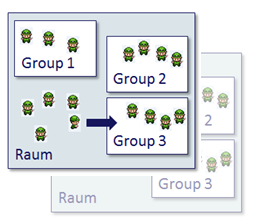
\includegraphics{graphiken/konzeptskizze.png}%
\caption{Konzeptskizze von Raum, Gruppen und Mitgliedern (Quelle: Eigene Darstellung)}%
\label{konzeptskizze}%
\end{figure}

Die Bewegung der eigenen Figur kann dabei mit den Pfeiltasten einer Tastatur oder mit Hilfe des Fingers per Drag'n'Drop auf mobilen Endgeräten erfolgen. Die technische Details zur Realisierung werden im Kapitel \ref{architektur_technologie} näher erläutert. 
\newline\newline
Des Weiteren existiert pro Raum ein Chatfenster, in dem die Mitglieder sich unterhalten können. Mögliche Gesprächsthemen wären bspw. die Findung eines Gruppennamens, der Gruppenzusammensetzung oder die Aufgaben einer möglichen Gruppe. Da keine persistente Speicherung der Gruppen sowie deren Mitglieder nach Verlassen des Raumes vorgesehen ist, ist eine Exportfunktion der angezeigten Gruppeninformationen vorhanden.


% !TEX root = ../Gruppenbildung.tex
\chapter{Prototyp}
\label{prototyp}

In diesem Kapitel wird auf zunächst auf die Architektur und die verwendeten Technologien näher eingegangen. Anschliessend wird anhand verschiedener Screenshots die Bedienung der Webanwendung erläutert.

\section{Architektur und Technologien}
\label{architektur_technologie}

Der \emph{groupfindr} Prototyp demonstriert die technische Machbarkeit einer skalierbaren real-time Anwendung mit \emph{socket.io}, exploriert die Darstellungs- und Interaktionsmöglichkeiten der interaktiven Grafikbibliothek \emph{EaselJS}, und verwendet einen Standardstack an Webtechnologien zur Umsetzung einer responsive Webapplikation.
\newline\newline
Die event-basierte Javascript Bibliothek socket.io\footnote{\url{http://socket.io/}} ermöglicht die bidirektionale Kommunikation zwischen Client und Server in Echtzeit und bildet die Basis für die groupfindr Funktionalität Bewegungen anderer Benutzer in Echtzeit zu verfolgen. Bewegt ein Benutzer seinen Avatar, wird seine neue Position (\code{pos}) über einen etablierten Websocket (\code{socket}) vom Client-Browser an den Server emittiert: \code{socket.emit('updatepos', pos);}. Der Server reagiert auf den updatepos Event mit dem in Listing 1 gezeigten Callback. Bei der Positionüberprüfung wird festgestellt ob der Benutzer durch die Positionsänderung soeben eine Gruppe verlassen oder betreten hat. Anschliessend wird die neue Position (\code{newPos}) an alle Benutzer im selben Raum gesendet.

\begin{lstlisting}[caption=Server Implementation des \emph{updatepos} Event]
socket.on('updatepos', function (pos) { 
  // ... 
  // Broadcast new position to all other player in the same room 
  app.io.to(pos.roomname).emit('update', newPos); 
  // ... 
}
\end{lstlisting}

Eine Herausforderung mit Echzeitkommunikation dieser Art ist die Sicherstellung einer konsistenten Sicht über alle verbundenen Benutzer. Durch die häufigen parallelen Updates können leicht Logikfehler im Event-Handling entstehen, die beispielsweise dazu führten, dass einzelne Benutzer dupliziert wurden. Des Weiteren hat die Terminologie von Räumen (\emph{rooms}) für etwas Verwirrung gesorgt, da dieser Begriff sowohl in der technischen (als socket.io Namensraum) als auch in der konzeptionellen (als virtuellen Raum in dem sich Gruppen bilden) Domäne existiert.
\newline\newline
Die in CreateJS enthaltene Javascript Bibliothek EaselJS verwenden wir zur dynamischen Darstellung des Raum Canvas und insbesondere zur Animation des beweglichen Benutzer-Avatars. Dafür bietet EaselJS\footnote{\url{http://www.createjs.com/easeljs}} einen eleganten Weg über sogennante SpriteSheets wie Abbildung~\ref{fig:spritesheet} illustriert. Listing~\ref{lst:spritesheet} zeigt wie diese einzelne Bilder oder eine Abfolge von Bildern für Bewegungen in bestimmte Richtungen mit einer konfigurierbaren Geschwindigkeit (\code{0.4}) konfiguriert werden können. Eine nennenswerte Herausforderung war die korrekte relative Berechnung der Positionskoordinaten beim skalieren des Raum Canvas.

\begin{figure}[htbp]
\begin{tabular}{p{0.45\textwidth}p{0.5\textwidth}}
    \begin{minipage}{.5\textwidth}
    \centering
    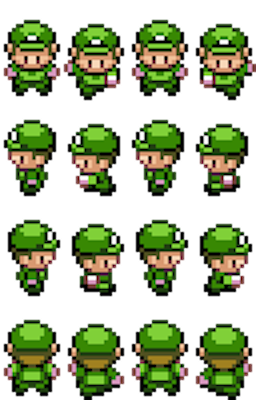
\includegraphics[width=0.45\linewidth]{graphiken/player.png}
    \caption{Avatar SpriteSheet}
    \label{fig:spritesheet}
    \end{minipage}
    &
    \begin{minipage}{.5\textwidth}
\begin{lstlisting}[caption=EaselJS Avatar Animationen,label=lst:spritesheet]
createjs.SpriteSheet({
  "images": [image],
  frames: {width: 64, height: 100, regX: 32, regY: 50, count: 16},
  animations: {
    "standdown": 0,
    "standleft": 4,
    "standright": 8,
    "standup": 12,
    "down": [1, 3, "standdown", 0.4],
    "left": [5, 7, "standleft", 0.4],
    "right": [9, 11, "standright", 0.4],
    "up": [13, 15, "standup", 0.4]
  }
});
\end{lstlisting}
\end{minipage}
\end{tabular}
\end{figure}

Groupfindr verwendet einen Standardstack an Webtechnologien zur Umsetzung einer response Webapplikation. Serverseitig kommt Node.js\footnote{\url{https://nodejs.org/}}, Express\footnote{\url{http://expressjs.com/}}, und die templating Engine Jade\footnote{\url{http://jade-lang.com/}} zum Einsatz. Die Websocket Verbingungen zwischen Client und Server werden durch socket.io abstrahiert. Clientseitig verwenden wir Bootstrap\footnote{\url{http://getbootstrap.com/}}, CSS, und Javascript mit den Bibliotheken EaselJS, jsPDF\footnote{\url{http://parall.ax/products/jspdf}}, und JQuery\footnote{\url{https://jquery.com/}}.
\newline\newline
Die ausklappbare Chatbox am unteren Bildrand (siehe Abbildung~\ref{groupfindr_einfaerbung-chat}) als Einfallstor für Injection Attacken auf alle Benutzer im gleichen Raum dienen. Chatnachrichten erlauben die Verwendung von HTML Tags (z.B. \code{<b>html</b>}). Während solch harmlose Formatierungen kein Problem darstellen, lässt sich durch die Verwendung eines HTML Skript-Tags beliebiger Code im Browser aller Benutzer ausführen wie das Beispiel in Abbildung \ref{groupfindr_einfaerbung-chat} zeigt. 
\newline
Das Senden der Chatnachricht \code{<script>window.location = "https://google.com";</script>} leitet alle Benutzer im gleichen Raum unmittelbar auf die Google Website weiter. Sicherheitskritische Attacken dieser Art lassen sich verhindern, indem der Server jede Chatnachricht überprüft und bevor der Weiterleitung an andere Benutzer alle HTML Elemente entsprechend escaped.

\section{How To}
\label{how_to}

Auf der Startseite der Groupfindr Web Applikation\footnote{\url{https://groupfindr.herokuapp.com/}} kann der Benutzer Benutzername und Raum auswählen (siehe Abbildung \ref{groupfindr_einstieg-gruppenerstellung}). Existierende Räume werden ihm dabei als Dropdown-Auswahl zur Verfügung gestellt. Sobald ein Benutzer einen virtuellen Raum (dargestellt als rechteckige begehbare Fläche) betritt, erhält er einen Avatar zugewiesen (siehe Abbildung \ref{groupfindr_einstieg-gruppenerstellung}). Im virtuellen Raum kann der Benutzer seinen Avatar über Pfeiltasten, per Maus, oder Touch-freundlich per Drag’n’Drop bewegen. Dabei kann jeder Benutzer die Laufwege aller Benutzer im gleichen Raum in Echtzeit mitverfolgen.

\begin{figure}
\centering
\begin{tabular}{cc}
\subfloat[Login Screen]{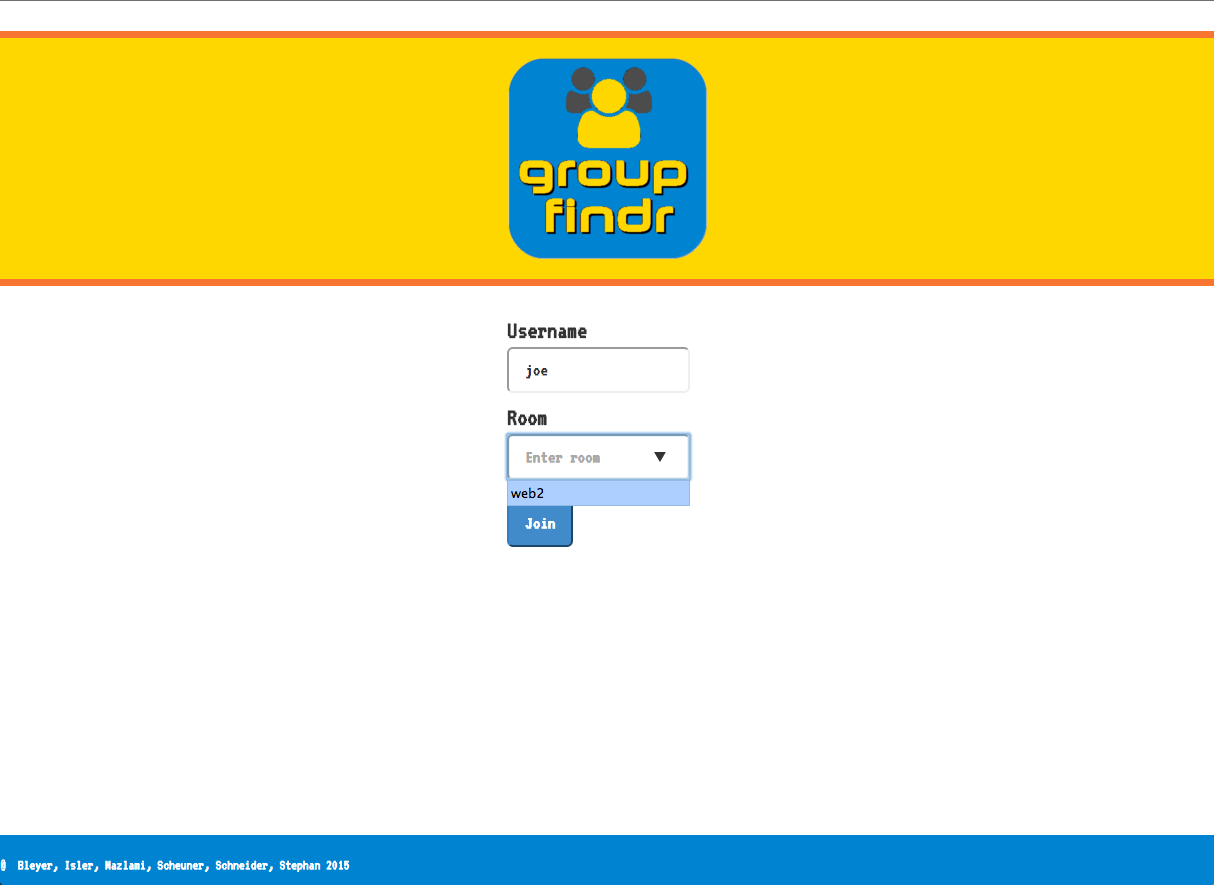
\includegraphics[width=0.3\linewidth]{graphiken/login.png}} & 
\multirow{-7}[9.3]{*}{\subfloat[Raum Beigetreten]{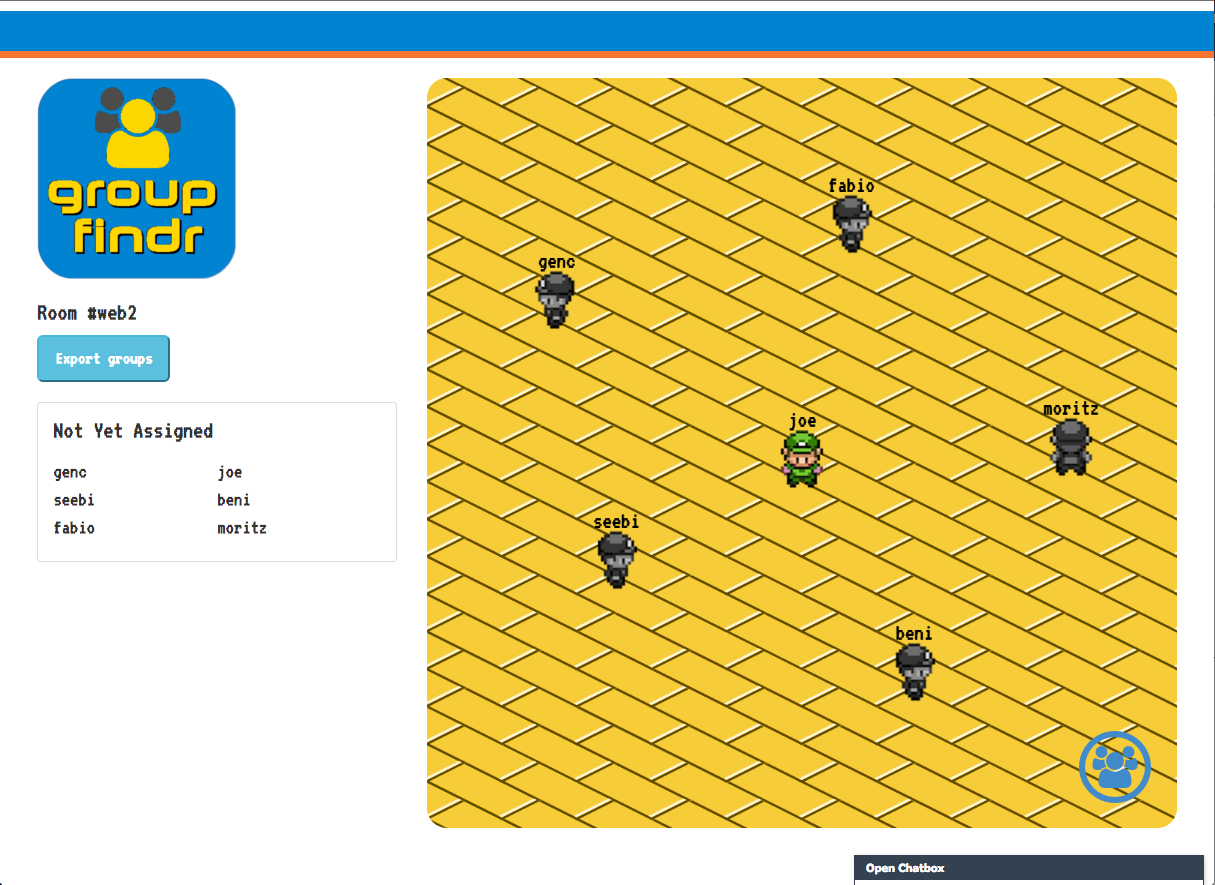
\includegraphics[width=0.6\linewidth]{graphiken/joined-canvas.png}}} \\
\subfloat[Gruppe Erstellen]{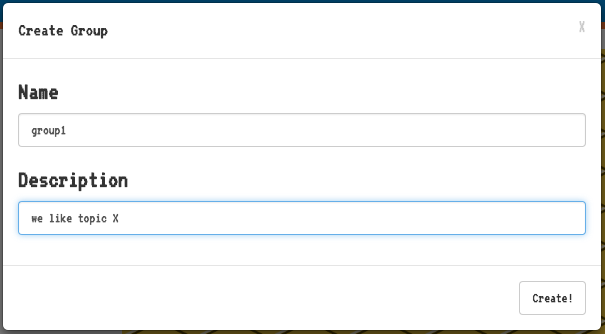
\includegraphics[width=0.3\linewidth]{graphiken/create-group.png}} &
\end{tabular}
\caption{Groupfindr - Einstieg \& Gruppenerstellung (Quelle: Eigene Darstellung)}
\label{groupfindr_einstieg-gruppenerstellung}
\end{figure}

\begin{figure}[h]
\centering
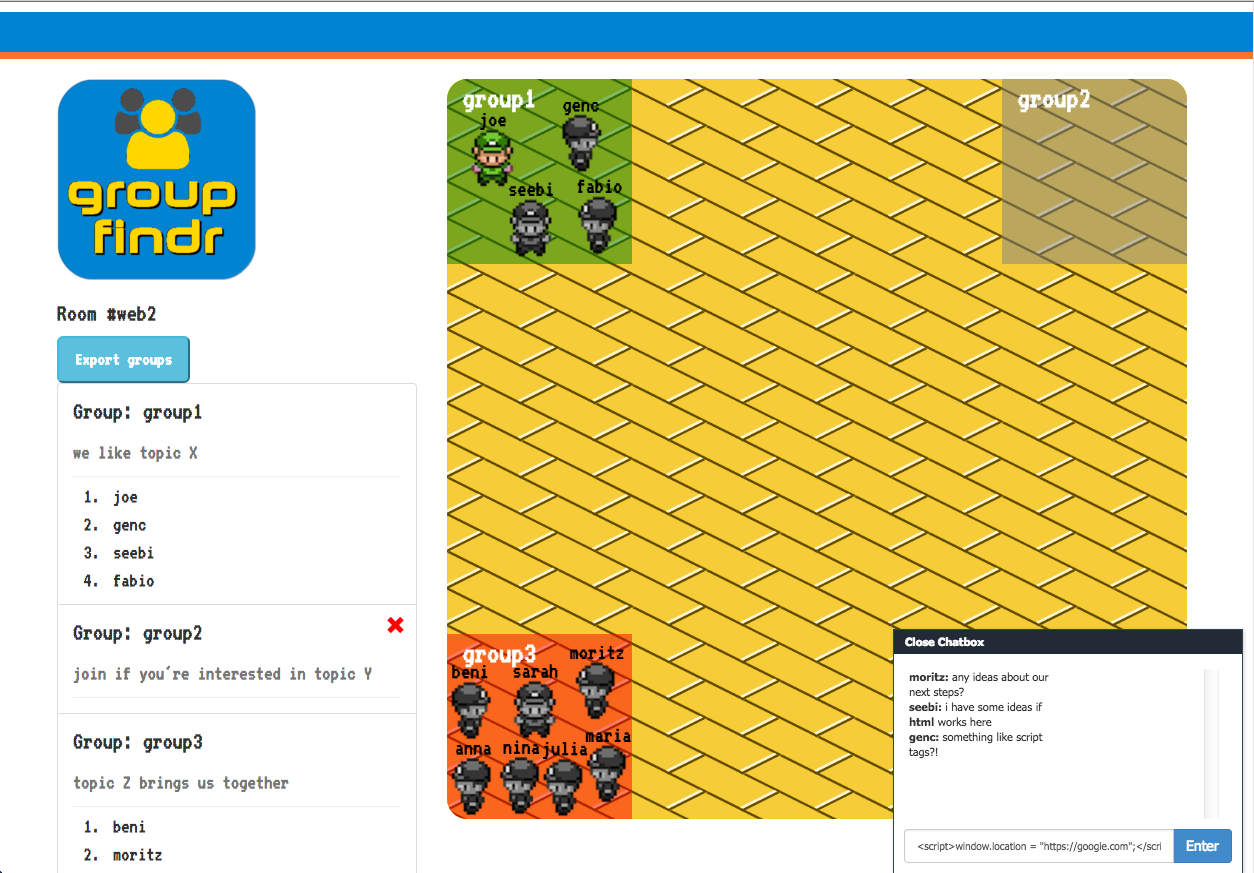
\includegraphics[width=\linewidth]{graphiken/groups-and-chat.png}
\caption{Groupfindr - Einfärbung der Gruppen und Chatbox (Quelle: Eigene Darstellung)}
\label{groupfindr_einfaerbung-chat}
\end{figure}

Solange noch freie Plätze auf dem Canvas bestehen (in diesem Prototyp aus Darstellungsgründen auf 7 begrenzt), kann jeder Benutzer über den blauen Gruppenbutton im Canvas eine neue Gruppe mit Namen und Beschreibung erstellen. Jeder Benutzer kann einer Gruppe betreten indem er seinen Avatar in das Feld der Gruppe seiner Wahl bewegt (siehe Abbildung~\ref{groupfindr_einstieg-gruppenerstellung}). Gruppen mit optimaler Mitgliederanzahl (4-6) werden dabei grün eingefärbt, solche mit zu vielen Mitgliedern sind an der roten Einfärbung schnell zu erkennen, siehe Abbildung~\ref{groupfindr_einfaerbung-chat}. Jeder Benutzer kann leere Gruppen wieder löschen um Platz für weitere Gruppen zu schaffen. Die aktuellen Gruppeneinteilungen sind jederzeit in einer textuellen Übersicht, links neben dem Canvas einsehbar. Diese Übersicht lässt sich am Ende des Gruppenfindungsprozesses über die Exportfunktion (Export groups) als PDF herunterladen.

\chapter{Business Case und Ausblick}
\label{business_case}

In Wirtschaft, Wissenschaft und Verwaltung existieren verschiedenen Methoden wie Gruppen gebildet werden können, bspw. nach dem Zufall, Interessen oder persönlichen Merkmalen wie der Geburtsmonat oder ähnlichem. Ausserdem existieren bereits eine Vielzahl von Softwareanwendungen, die die Organisation der Prozesse innerhalb eine Gruppe unterstützen. Als Beispiele können hier verschiedene Kollaborationsanwendungen im Unternehmenskontext oder auch Facebook, Google+ oder WhatsApp im privaten Bereich aufgeführt werden. Den Autoren ist jedoch keine Anwendung bekannt die ihren Fokus auf die schnelle und einfache Bildung von Gruppen in Echtzeit legt: ein Doodle für die Gruppenfindung. 

\begin{figure}[h]
\centering
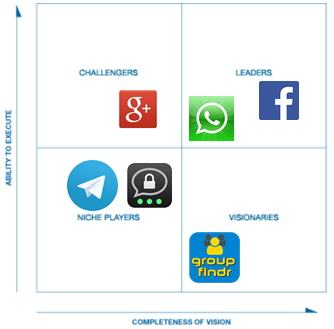
\includegraphics[width=0.5\linewidth]{graphiken/magic_quadrant.png}%
\caption{Einordnung und Vergleich des \emph{groupfindr} mit Mitbewerbern (Quelle: Eigene Darstellung)}%
\label{magic_quadrant}%
\end{figure}

Auch wenn der Schwerpunkt des \emph{groupfindr} nicht auf die Unterstützung der Gruppenprozesse liegt, wurden dennoch verschiedene soziale Plattformen mit dem \emph{groupfindr} mit Hilfe der Magic Quadrant Methode der Gartner Group \citet{magic_quadrant} verglichen, siehe Abbildung \ref{magic_quadrant}.  Die Merkmale, die für die Einordnung herangezogen wurden, sind \citet{gruppen-bildung} entnommen und durch die subjektive Einschätzung der Autoren ergänzt worden. Nach der Meinung der Autoren ist die \emph{groupfindr} Anwendung im Bereich der Visionären einzuordnen, da das Hauptaugenmerk auf Funktionalitäten liegt die durch die Mitbewerber nicht berücksichtigt werden. Allerdings ist der Funktionsumfang im Hinblick auf die Organisation und Kommunikation innerhalb der Gruppe nur sehr eingeschränkt.
\newline\newline
Eine Vermarktung des \emph{groupfindr} ist mit zwei verschiedenen Lizenzvarianten denkbar. In der ersten Variante wird eine OnDemand oder Cloudlösung angeboten, die jeder kostenfrei nutzen kann. Eine Finanzierung könnte hierbei durch Werbung erfolgen. Außerdem wäre auch die Erweiterung um Benutzerprofile denkbar, um mit den dann verfügbaren Daten passendere Werbung bereitstellen zu können. Es ist ebenfalls denkbar für verschiedene Bildungsinstitutionen wie Universitäten oder Schulen eine werbefreie Version der Cloudlösung gegen eine Lizenzgebühr anzubieten, die dann auch an spezifische Bedürfnisse angepasst werden könnte. Die zweite Variante wäre, dass die komplette Anwendung von den Käufern selbstständig betrieben wird (OnPremise Variante). Dies könnte insbesondere für Karrierenetzwerke wie XING oder LinkedIn interessant sein, um die Bildung von Projektteams für bereits auf den Plattformen ausgeschriebenen Projekten zu vereinfachen, ohne die Daten der Profile der eigenen Plattformen weitergeben zu müssen. Auch hier wäre dennoch eine Lizenzgebühr oder ggf. auch ein einmaliger Kaufpreis denkbar.
\newline\newline
Mit der jetzigen Version der Anwendung \emph{groupfindr} konnte das Problem der einfache und schnelle Gruppenbildung in Echtzeit gelöst werden. Auch wenn der momentane Schwerpunkt auf die Gruppenbildung im Rahmen von Vorlesungen im Hochschulstudium liegt, ist ein Ausbau und kommerzielle Vermarktung aus Sicht der Autoren sinnvoll und machbar.



% Literaturliste endgueltig anzeigen
%\bibliography{bibliographie/literatur}
%\bibliographystyle{jurabib}
\printbibliography

\end{document}
